\documentclass[10pt,french]{book}

\input preambule_2013
\pagestyle{empty}

\usepackage{geometry} % package offrant une autre méthode pour redéfinir les marges
\geometry{a4paper, top=1cm,bottom=1cm,left=1cm,right=1cm}

\newcommand\presentation{
    \begin{tabular}{ll}
        Nom : \\[5pt]
        Prénom :
    \end{tabular}
\hfill
    \textbf{Note :}
        \renewcommand\arraystretch{2.3}
    \begin{tabular}{|c|}
        \hline
            \slashbox{\Huge\bfseries\phantom{10}}{\Huge\bfseries 10}\\
        \hline
    \end{tabular}
        \renewcommand\arraystretch{1.5}\par
    \vspace{1cm}
    \hrulefill
}


\begin{document}

\begin{landscape}
\presentation

\begin{multicols}{2}
\small
Dans un repère \OIJ, on a tracé la courbe $\calig C_f$ représentative de la fonction $f$.\medskip


\begin{description}
    \item[Partie A :] \textit{Par lecture graphique.}
       \begin{enumerate}
            \item Déterminer $f(0)$ et $f(-1)$.
            \item Donner une valeur approchée des antécédents de $0$.
            \item Combien d'antécédents possède le nombre $-1$ ? et le nombre $2,75$ ?
            \item Quels sont tous les nombres qui ont $3$ antécédents par $f$ ? Donner la réponse sous forme d'un intervalle.
        \end{enumerate}
    \item[Partie B :] \textit{Par calcul numérique.}\par
    La fonction $f$ est définie pour tout $x \in \R$ par \[f(x) = 2x^3 -x^2 - 4x + 1.\]
        \begin{enumerate}
            \item Le point $E$ de coordonnées $(-1,25 \pv 0,5)$ appartient-il à $\calig C_f$ ? Justifier la réponse.
            \item Développer $(x - 1)^2$.
            \item Démontrer que $f(x) = (2x+3)(x-1)^2-2$.
            \item En déduire les antécédents de $-2$ par la fonction $f$.
            \item En détaillant précisément les étapes, l'image de $\frac{-1}{2}$ par la fonction $f$.
        \end{enumerate}
\end{description}

\begin{center}
    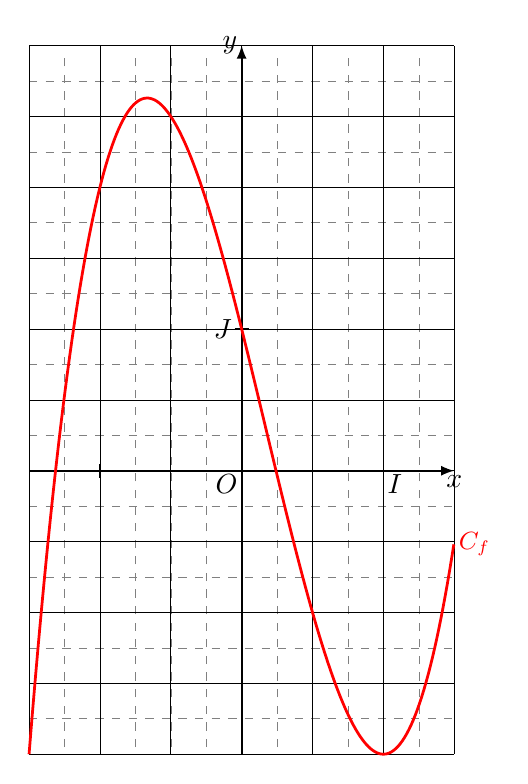
\begin{tikzpicture}[>=latex,y=2cm,x=2cm,scale=0.9]
        \draw[help lines, dashed] (-1.5,-1.95) grid[step=0.5cm] (1.5,2.95);
        \draw[line width = 0.25pt] (-1.5,-2) grid (1.5,3);
        \draw[->,line width = 0.65pt] (-1.5,0) -- (1.5,0) node[below=-2pt] {$x$};
        \draw[->,line width = 0.65pt] (0,-2) -- (0,3) node[left=-2pt] {$y$};
        \coordinate (O) at (0,0); \draw (O) node[below left = -2pt] {$O$};
        \coordinate (I) at (1,0); \draw (I) node[below right = -2pt] {$I$}; \foreach \x in {-1,...,1}  \draw (\x,-0.05)--(\x,0.05);
        \coordinate (J) at (0,1); \draw (J) node[left] {$J$}; \foreach \x in {-1,...,2} \draw (-0.05,\x)--(0.05,\x);
        \draw[color=red,line width=1pt] plot[domain=-1.5:1.5,samples=200] (\x,{(\x-1)^2*(2*\x+3)-2}) node[right=-2pt] {\small $\calig C_f$};
    \end{tikzpicture}
\end{center}

\columnbreak

\textbf{Réponses :}

\end{multicols}


\clearpage

%--------------------------------------------------------------------------------------------------------------------------------------------------------------------------
%                           SUJET B
%--------------------------------------------------------------------------------------------------------------------------------------------------------------------------

\presentation

\begin{multicols}{2}
\small
Dans un repère \OIJ, on a tracé la courbe $\calig C_f$ représentative de la fonction $f$.\medskip


\begin{description}
    \item[Partie A :] \textit{Par lecture graphique.}
       \begin{enumerate}
            \item Déterminer $f(0)$ et $f(1)$.
            \item Donner une valeur approchée des antécédents de $0$.
            \item Combien d'antécédents possède le nombre $1$ ? et le nombre $-2,25$ ?
            \item Quels sont tous les nombres qui ont $3$ antécédents par $f$ ? Donner la réponse sous forme d'un intervalle.
        \end{enumerate}
    \item[Partie B :] \textit{Par calcul numérique.}\par
    La fonction $f$ est définie pour tout $x \in \R$ par \[f(x) = 2x^3 -7x^2 + 4x + 2.\]
        \begin{enumerate}
            \item Le point $E$ de coordonnées $(-0,25 \pv 0,5)$ appartient-il à $\calig C_f$ ? Justifier la réponse.
            \item Développer $(x - 2)^2$.
            \item Démontrer que $f(x) = (2x+1)(x-2)^2-2$.
            \item En déduire les antécédents de $-2$ par la fonction $f$.
            \item En détaillant précisément les étapes, l'image de $\frac{1}{2}$ par la fonction $f$.
        \end{enumerate}
\end{description}

\begin{center}
    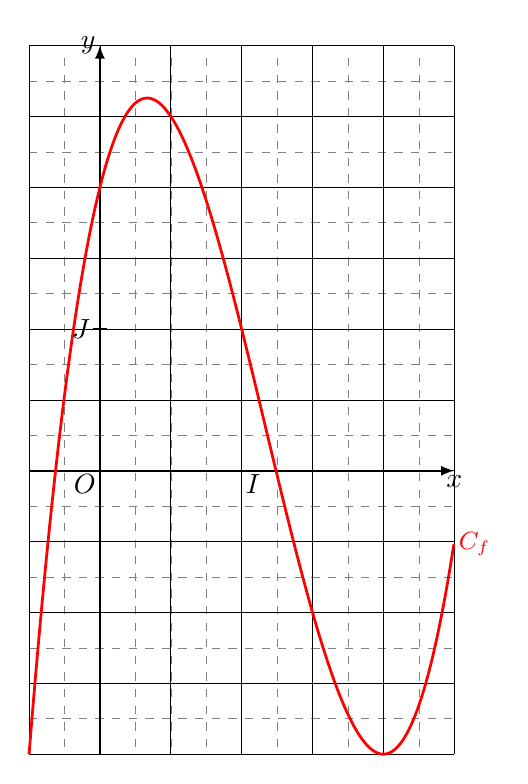
\begin{tikzpicture}[>=latex,y=2cm,x=2cm,scale=0.9]
        \draw[help lines, dashed] (-0.5,-1.95) grid[step=0.5cm] (2.5,2.95);
        \draw[line width = 0.25pt] (-0.5,-2) grid (2.5,3);
        \draw[->,line width = 0.65pt] (-0.5,0) -- (2.5,0) node[below=-2pt] {$x$};
        \draw[->,line width = 0.65pt] (0,-2) -- (0,3) node[left=-2pt] {$y$};
        \coordinate (O) at (0,0); \draw (O) node[below left = -2pt] {$O$};
        \coordinate (I) at (1,0); \draw (I) node[below right = -2pt] {$I$}; \foreach \x in {0,...,2}  \draw (\x,-0.05)--(\x,0.05);
        \coordinate (J) at (0,1); \draw (J) node[left] {$J$}; \foreach \x in {-1,...,2} \draw (-0.05,\x)--(0.05,\x);
        \draw[color=red,line width=1pt] plot[domain=-0.5:2.5,samples=200] (\x,{((\x-1)-1)^2*(2*(\x-1)+3)-2}) node[right=-2pt] {\small $\calig C_f$};
    \end{tikzpicture}
\end{center}

\columnbreak

\textbf{Réponses :}

\end{multicols}
\end{landscape}

\end{document} 